\documentclass[german,seminar]{KITthesis}

\title{\Huge Hybrider OP-Saal}
\titleotherlanguage{Hybrid Operating Room}

\author{Theresa Heine}
\address{Brauerstraße 19}
\city{76137 Karlsruhe}
\email{uuecn@student.kit.edu}

\keywords{Hybrider OP-Saal, Netzwerkkommunikation, Datenaustausch, Herausforderungen}
\keywordsotherlanguge{Hybrid Operating Room, Network Communication, Data Exchange, Challenges}

\studyprogram{\LARGE Informatik in der Medizin}

\reviewerone{Prof. Dr.-Ing. Torsten Kröger}
\reviewertwo{Prof. Dr.-Ing. habil. Björn Hein}

\advisorone{M.Sc. Christian Marzi}
% %% The second advisor can be omitted
\advisortwo{M.Sc. D}

\editingtime{16. April 2018}{18. Juni 2018}

\usepackage{graphicx}
\usepackage[format=plain, indention=0cm]{caption}
\usepackage{babel,blindtext}

\settitle

\begin{document}

\setpdf
\includetitle
\includedeclaration
\includeacknowledgments


\inculdetableofcontents

\makenomenclature

\setmainpart

\chapter{\iflanguage{ngerman}{Übersicht Hybrider OP-Saal}{Overview}}
\label{sec:overview}

Weniger invasive Eingriffe, geringeres Risiko und kürzere Operations-und Krankenhausaufenthalte sind Anforderungen die heutzutage an Ärzte und Operationssäle gestellt werden \cite{DerDigitaleOperationssaal}. Anforderungen, welchen ein konventioneller OP-Saal nicht mehr gerecht werden kann. Aus diesem Grund findet ein Umstieg zum Hybriden/ Digitalen/ Multifunktionalen oder auch Hochpräzisions OP-Saal statt. Unabhängig der Bezeichnung, geht es darum den OP-Saal zu digitalisieren und Bildgebende Verfahren wie Röntgen oder Ultraschall während der Operation einzusetzen.

In den folgenden Kapiteln wird immer vom Hybriden OP-Saal die Rede sein und es werden die Unterschiede vom Hybriden zum Konventionellen OP-Saal herausgearbeitet, sowie in welchen Einsatzgebieten der Hybride OP-Saal bereits verwendet wird und welche Vorteile dieser mit sich bringt.

\subsection{Hybrider OP-Saal vs. Konventioneller OP-Saal} 

\begin{figure} [H]
	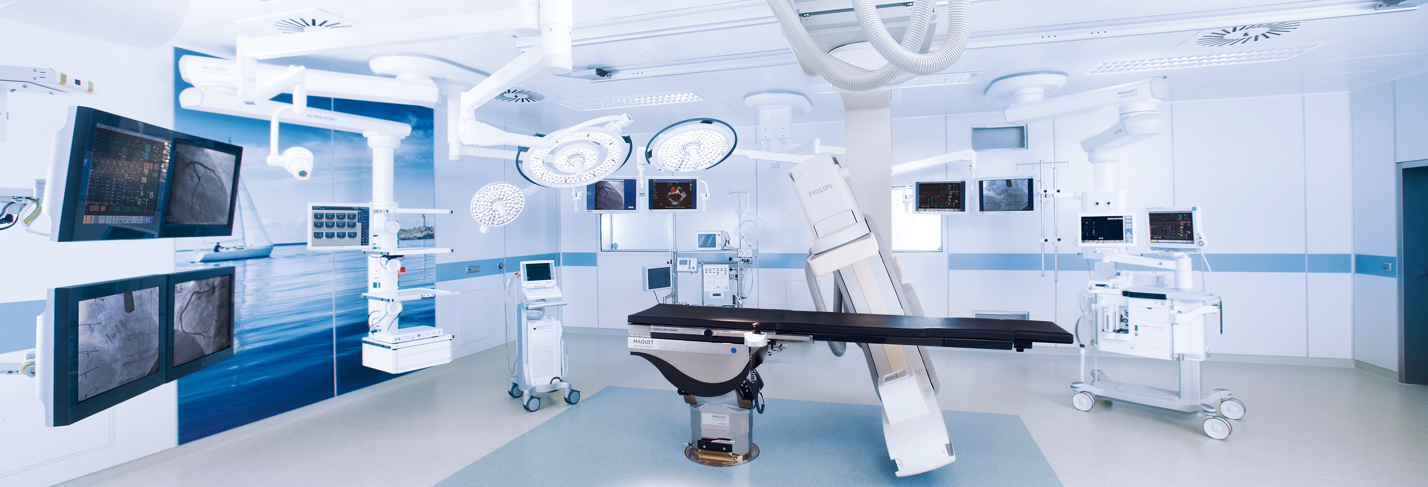
\includegraphics[scale = .3]{Content/Pictures/hybrid-or.png}
	\caption{Hybrider OP-Saal von Maquet mit einem an der Decke fixierten C-Bogen \cite{Maquet}.}
	\label{fig:hybridor}
\end{figure}

Ein Hybrider OP-Saal (Beispiel in Abb. \ref{fig:hybridor}) ist die Kombination aus einem sterilen konventionellen OP-Saal mit qualitativ hochwertiger Bildgebung. Hinzu kommt ein multifunktionalen OP-Tisch, digitale Datenregistrierung und Dokumentation sowie ungehinderter Datenaustausch innerhalb und außerhalb des OPs. Zur Steuerung und Kontrolle der Geräte und Systeme im OP-Saal steht ein Interface zur Verfügung \cite{HybriderVsKonventioneller,KarlStorz}. Darüber hinaus ist ein Hybrider OP-Saal, gegenüber einem Konventionellen OP-Saal, ein fachbereichsübergreifender chirurgischer Arbeitsbereich. Er wird gleichermaßen von der Neurochirurgie, Gefäßchirurgie, Onkologie, Kardiologie, Unfallchirurgie und vielen weiteren Bereichen genutzt \cite{Getinge}.\\
Mobile C-Bogen sowie Ultraschall- und Endoskopiegeräte gehören zur Standardausrüstung in Konventionellen OP-Sälen \cite{TechnicalConsiderations}. Für komplexe Operationsvorgänge wie bspw. bei Transkathetertechniken und für die Visualisierung der dünnen Führungsdrähte, wird jedoch eine leistungsstärkere Ausrüstung benötigt. Aus diesem Grund werden die mobilen C-Bogen durch befestigte ersetzt. Zur ergänzenden Ausrüstung des Hybriden OP-Saals können noch weitere Geräte für die intraoperative Bildgebung, wie Computertomographen (CT), Magnetresonanztomographen (MRT) oder Angiografieanlagen gehören \cite{OPderZukunft}. 
Die befestigten C-Bogen ermöglichen qualitativ hochwertige Echtzeitbildgebung mit Fluroskopie (Abb. \ref{fig:fluroscopy}) mit deren Hilfe Katheter durch den Körper geführt werden können. Ein Weiteres Verfahren ist die Digitale Subtraktionsangiographie (Abb. \ref{fig:dsa}). Dabei werden zwei Bilder vom jeweilig abzubildenden Gebiet, einmal mit und einmal ohne Kontrastmittel, angefertigt. Bei Subtraktion der beiden Bilder bleiben die Blutgefäße mit dem Kontrastmittel zurück \cite{CurrentAndFuture}. Darüber hinaus bieten MRT und CT die Möglichkeit hochauflösende Bilder von Geweben und Organen anzufertigen (Abb. \ref{fig:mrtct}).\\

\begin{figure}[!htb]
	\minipage{0.32\textwidth}
	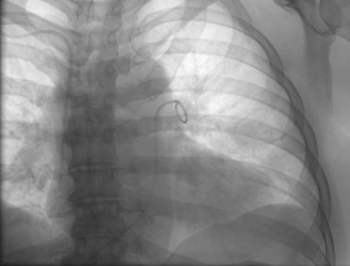
\includegraphics[width=\linewidth]{Content/Pictures/fluroscopy.png}
	\caption{Fluroskopie Aufnahme durch einen C-Bogen \cite{CurrentAndFuture}.}
	\label{fig:fluroscopy}
	\endminipage\hfill
	\minipage{0.32\textwidth}
	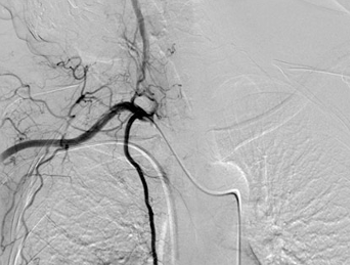
\includegraphics[width=\linewidth]{Content/Pictures/dsa.png}
	\caption{2D Bild mit Digitaler Subtraktionsangiographie (DSA) \cite{CurrentAndFuture}.}
	\label{fig:dsa}
	\endminipage\hfill
	\minipage{0.32\textwidth}%
	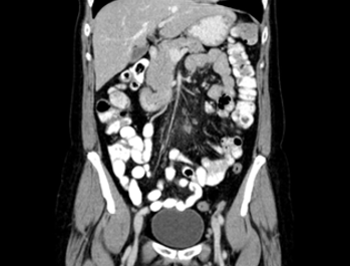
\includegraphics[width=\linewidth]{Content/Pictures/mrtct.png}
	\caption{CT-Aufnahme des Magens und Zwölffingerdarms \cite{CTBild}.}
	\label{fig:mrtct}
	\endminipage
\end{figure}

Somit können während eines Operationsvorgangs Diagnose und Therapiekontrolle vorgenommen, sowie minimal invasive Behandlungsverfahren durchgeführt werden \cite{SHG-Kliniken}. Auch ist es möglich \glqq während der Operation - und nicht erst danach - Bildkontrollen durch[zu]führen und allenfalls Korrekturmaßnahmen [zu] ergreifen\grqq{} \cite{OPderZukunft}. 

\subsection{Vorteile und wichtige Einsatzgebiete}

Wie Hybride OP-Säle Operationsvorgänge unterstützen, soll in der Neurochirurgie anhand der Kompensation des Brain Shifts, in der Gefäßchirurgie anhand des Setzens von Prothesen bei Aortenaneurysmen und in der Onkologie anhand der Tumorentfernung, erklärt werden.

\textbf{Neurochirurgie:}
Das Gehirn ist eine komplexe dreidimensionale Struktur, bei der sogenannte Brain Shifts (Verschiebungen der Gehirnstruktur Abb. \ref{fig:brainshift}) während einer Operation auftreten können. Ursachen für Brain Shifts können die Entfernung oder das Anschwellen von Gewebe, sowie der Verlust von Hirnwasser sein. Kommt es während einer Operation zu den oben genannten Verschiebungen, dann stimmen die vor einer Operation angefertigten CT- oder MR-Bilder der Gehirnstruktur nicht mehr mit der aktuellen Struktur überein. Bild geführte neurochirurgische Systeme (Image Guided Neurosurgical Systems, kurz IGNS), die während der Operation als Navigationshilfe dienen, können wegen den inkorrekten Bilddaten nur noch begrenzt arbeiten \cite{BrainShiftInTumorResection}.\\
Intraoperativer Ultraschall (iUS) oder intraoperative MR-Bilder (iMR) können diesem Problem entgegenwirken und die fehlenden Informationen ergänzen, sodass das IGNS wieder einsetzbar ist. IMR ermöglicht, während der Operation regelmäßig hochauflösende Bilder von der Gewebestruktur des Gehirns anzufertigen. Im Falle eines Brain Shifts kann dann entsprechend reagiert werden. Auch bei anderen neurochirurgischen Anwendungen wie der Hirnbiopsie, Entfernung von Tumoren oder der Drainage von Zysten kann iMR von Vorteil sein \cite{BrainShiftInTumorResection}.\\
Obwohl iMR als verlässlichste Option gilt, Bilder vom Gehirn anzufertigen und Brain Shifts zu erkennen, hat iUS den Vorteil kostengünstig Echtzeitzeitbilder zu produzieren. Die Kombination aus einem präoperativen MR-Bild und iUS reicht aus, um Gewebeveränderungen zu registrieren und die Korrektheit des IGNSs zu beurteilen. Im Gegensatz zu iMR, mit einer Bildaufnahmezeit von 15 Minuten, kann ein iUS-Bild in 5 Minuten aufgenommen werden. Aufgrund der vergleichbar schlechten Bildqualität gegenüber iMR wird iUS bisher begrenzt in der Neurochirurgie verwendet. Neue Ansätze (siehe Kapitel 4.1) ermöglichen jedoch die Möglichkeit einer genaueren US-Bildgebung für diesen Bereich \cite{BrainShiftInTumorResection}.

\begin{figure}[!htb]
	\minipage{0.45\textwidth}
	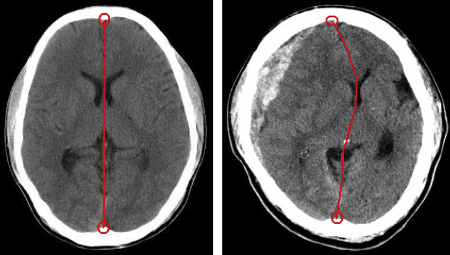
\includegraphics[width=\linewidth]{Content/Pictures/brainshift.png}
	\caption{(links) Keine Verschiebung, (rechts) Verschiebung der Mittellinie des Gehirns (midline brain shift) durch Anschwellen von Gewebe \cite{BrainShiftImage}.}
	\label{fig:brainshift}
	\endminipage\hfill
	\minipage{0.45\textwidth}%
	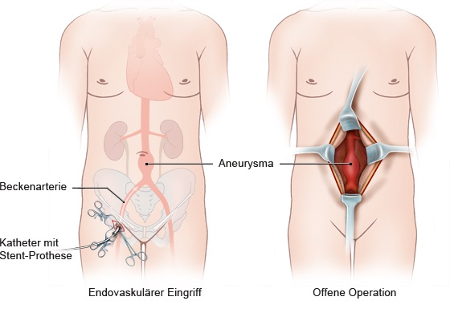
\includegraphics[width=\linewidth]{Content/Pictures/bauchaorten.png}
	\caption{(links) Endovaskulärer Eingriff bei einem Bauchaortenaneurysma mit Stent-Prothese gegenüber (rechts) einer offenen Operation mit normalen Prothesen \cite{BauaortenaneurysmaBild}.}
	\label{fig:bauchaorten}
	\endminipage
\end{figure}

\textbf{Gefäßchirurgie:}
Die Gefäßchirurgie profitiert von Hybriden OP-Sälen durch intraoperative Echtzeitbildgebung. Diese erlaubt den Fortschritt eines Katheters durch die Gefäße zu beobachten. Dadurch können das Ergebnis, wie das Setzen und richtige Sitzen einer Prothese, beurteilt werden \cite{DresdnerUniklinikum,TickendeBombeImBauch}. In Bezug auf ein Aortenaneurysma, eine krankhafte Erweiterung der Hauptschlagader, ergeben sich alternative Möglichkeiten der Operationsdurchführung. Da Aortenaneurysmen ruptieren und zu lebensbedrohlichen Blutungen führen können, muss ab einem gewissen Durchmesser der Erweiterung eine Prothese gesetzt werden \cite{Aortenaneurysma}. Die Operation kann entweder als offene Operation mit konventionellen Prothesen durchgeführt werden oder mit einem schonenden Verfahren und Implantation großer maßgefertigter Gefäßprothesen im Hybriden OP-Saal (siehe Abb. \ref{fig:bauchaorten}) \cite{DresdnerUniklinikum}. \\
Die offene Operation, bei der bei Bauchaneurysmen ein großer Schnitt in die Bauchdecke gemacht werden muss, weist gute Langzeitergebnisse auf, ist aber belastet und mit vergleichsweise langen Erholungszeiten verbunden \cite{TickendeBombeImBauch}. Da Aortenaneurysmen verstärkt im höheren Alter (> 60 Jahre) auftreten, kommt für diese Patienten eine offene Operation nicht mehr in Frage \cite{Aortenaneurysma}. \\
Alternativ wird deshalb beim schonenden Verfahren vor der Operation ein CT Bild angefertigt, welches dann mit den während der Operation entstehenden zwei- oder dreidimensionalen Bildern der Röntgenkontrolle kombiniert wird. Dies ermöglicht eine Stent-Prothese minimalinvasiv einzusetzen. Mithilfe eines Katheters kann dabei über einen kleinen Zugang in der Leiste durch das abgebildete Gefäß navigiert werden. Eine zusätzliche Software zur Navigationshilfe trägt dazu bei, die Prothese durch die Gefäße ans Ziel zu bringen \cite{DresdnerUniklinikum,TickendeBombeImBauch}.

\textbf{Onkologie:}
In der Onkologie hat man im Hybriden OP-Saal den Vorteil, dass nachdem ein Tumor entfernt und bevor die Operation abgeschlossen wurde, ein Kernspin mit dem MRT gemacht werden kann. Ohne den Patienten zu transportieren kann sichergestellt werden, dass tatsächlich keine Rückstände des Tumors übersehen wurden. Sollte dem nicht der Fall sein, kann direkt nachkorrigiert werden. Durch diese Korrekturmöglichkeit können Folgeoperationen erspart bleiben \cite{AerzteZeitung}. In mehr als einem drittel der Fälle, in denen die vollständige Entfernung eines Tumors angenommen wurde, wurden mit iMR noch Rückstände festgestellt und nachkorrigiert \cite{BrainShiftInTumorResection}.

\textbf{Fazit:} Zusammenfassend ermöglicht der Hybride OP-Säle präziseres, sicheres und schonenderes operieren durch minimalinvasive Eingriffe, welche weniger belastend für den Patienten sind \cite{DresdnerUniklinikum}. Das wiederum  führt zu kürzeren Krankenhausaufenthalten und zu Kosteneinsparungen in der Nachbetreuung und -behandlung. Der beliebig positionierbare OP-Tisch in Kombination mit dem hochbeweglichen C-Bogen sorgen für bestmögliche Röntgenbildaufnahmen. Diese können zur Unterstützung vor, während und nach der Operation eingesetzt werden \cite{DresdnerUniklinikum}. Entscheidungen über den Fortlauf der Operation können so besser getroffen werden, Ergebnisse beurteilt und gegebenenfalls nachkorrigiert werden.


\chapter{\iflanguage{ngerman}{Netzwerkkommunikation und Datenaustausch}{Network communication}}
\label{sec:overview}

Ein digitaler Datenbus der alle Daten in Echtzeit zu Verfügung stellt und die Steuerung der medizinischen Geräte im OP-Saal über einen zentralen Zugriffspunkt, ist noch nicht die Realität. Netzwerkkommunikation und Datenaustausch zwischen den medizinischen Geräten im OP-Saal werden durch herstellerabhängige Schnittstellen eingeschränkt. Bei der Installation eines Hybriden OP-Saals, muss im Voraus ein Hersteller gewählt werden, denn \glqq eine Integration von Drittanbieterkomponenten kann nur in Kooperation mit dem Hersteller des Integrationssystems erfolgen\grqq{} \cite{DerDigitaleOperationssaal}.

Um diesem Problem entgegen zu wirken, wurde für eine herstellerübergreifende Netzwerkkommunikation die Service Oriented Architecture für den medizinischen Gebrauch angepasst. Des Weiteren sollen Standards wie DICOM, HL7 und IHE zum ungehinderten Datenaustausch beitragen.

\subsection{Service Oriented Architecture}

\begin{figure} [H]
	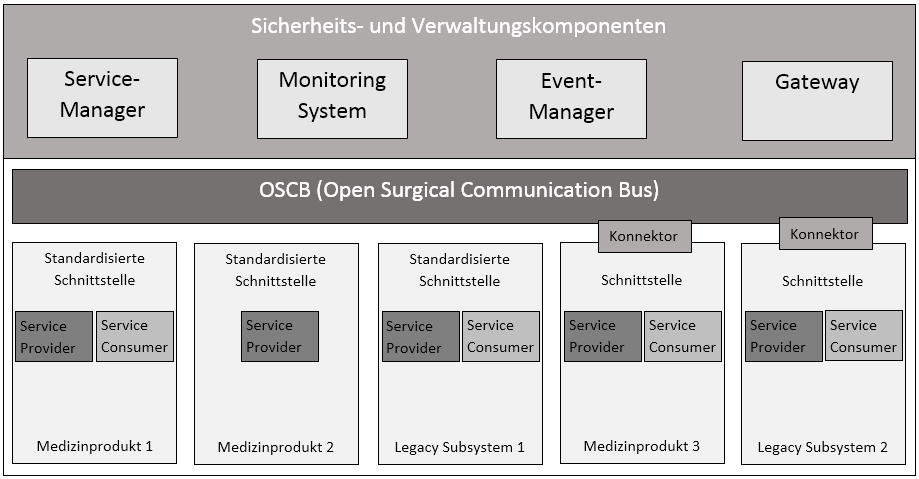
\includegraphics[scale = 0.6]{Content/Pictures/soa-red.png}
	\caption{SOA für den medizinischen Gebrauch im Operationssaal nach Abbild \cite{DerDigitaleOperationssaal}.}
	\label{fig:soa}
\end{figure}

In der Service Oriented Architecture (SOA, Abb. \ref{fig:soa}) für den medizinischen Gebrauch, interagieren Service Provider und Service Consumer über einen Open Surgical Communication Bus (OSCB). Dabei können medizinische Geräte sowohl Service Provider als auch Consumer sein und Dienste über eine standardisierte Schnittstelle nutzen bzw. bereitstellen. Der Service Manager verwaltet alle verfügbaren Geräte und Dienste im Netzwerk. Service Consumer können über den Service Manager Dienste anfragen, welcher verfügbare und passende Service Provider zur Verfügung stellt. Die Kommunikation läuft daraufhin direkt zwischen Consumer und Provider ab \cite{DerDigitaleOperationssaal}. \\ 
Für den Informationsaustausch sind standardisierte herstellerübergreifende Schnittstellen essentiell. Für Geräte die keine standardisierte Schnittstelle (wie DICOM) zu Verfügung stellen, übernimmt ein Konnektor die Aufgabe der Transformation. Damit wird eine höhere Bandbreite an Geräten unterstützt, welche in die SOA integriert werden können. Jegliche Kommunikation über den OP-Saal hinaus mit anderen Klinik-IT Netzwerken, wird über eine Gateway geleitet. So können die vorschriftsgemäßen Sicherheitsansprüche gewährleistet werden. Weitere optionale Komponenten sind der Event Manager und das Monitoring System. Der Event Manager verwaltet auftretende Ereignisse und informiert gegebenenfalls andere Geräte über diese. Das Monitoring System ist zur Unterstützung des Service Managers, für die Überwachung der angeschlossenen Geräte und um gegebenenfalls fehlerhafte Services zu identifizieren \cite{DerDigitaleOperationssaal}. 

Webservices bieten sich durch ihre lose Client-Server-Kopplung und Erweiterbarkeit für die Umsetzung der SOA im medizinischen Bereich an. Zur Verwirklichung des OSCBs ist Ethernet, aufgrund der hohen Bandbreite und der bereits bestehenden Infrastruktur in Krankenhäusern, die Grundlage für die Vernetzung. Die Gewährung der Sicherheit und Zuverlässigkeit des Systems ist mit einem höheren Aufwand verbunden als bei anderen Technologien. Die tatsächliche Client-Server-Kommunikation wird dann je nach Anwendungsfall mit TCP oder UPD verwirklicht \cite{DerDigitaleOperationssaal}.

Dieser Ansatz der Umsetzung einer SOA im medizinischen Umfeld, ermöglicht alle Geräte im Netzwerk über einen zentralen Zugriffspunkt im Operationssaal zu kontrollieren. Dazu gehören die bildgebenden Verfahren, aber auch der OP-Tisch, die Beleuchtungsanlagen und die Kameras mit der Anzeigeausgabe auf den Monitoren \cite{DerDigitaleOperationssaal}.

OR.NET (Secure Dynamic Networking in Surgery and Clinic) ist ein Projekt welches auf der SOA basiert und die Integration von medizinischen Geräten und IT-Systemen demonstriert. Ziel ist es, die Gerätekommunikation im OP zu erleichtern indem  Echtzeitkommunikation ermöglicht und eine internationale Normung für alle OP-Säle festgelegt wird. Zur Umsetzung dieses Projekts wurde ein Substandard entwickelt. Dieser soll nicht bereits vorhandene Standards wie HL7 oder DICOM ersetzen, sondern Geräte und Systeme in das IT-Netzwerk einbinden, welche die genannten Standards nicht umsetzen können \cite{ORnetWebsite}.\\
Zur Demonstration der Funktionsweise und Umsetzbarkeit von OR.NET wurden OP-Säle errichtet (Abb. \ref{fig:ornet}), die medizinische Geräte und klinische IT-Systeme von unterschiedlichen Herstellern vereinen \cite{ORnet}. Damit konnte gezeigt werden, dass eine einheitliche Mensch-Maschine-Interaktion unabhängig vom Hersteller möglich ist. Durch die Vernetzung kann während einer Operation auf präoperativ angefertigte Bilddateien, Patienteninformationen und Laborbefunde zugegriffen werden. Auch von außerhalb des OP-Saals können die Informationen eingesehen werden, die im OP-Saal erfasst und aufgezeichnet wurden \cite{ORnetWebsite}.

\begin{figure} [t!]
	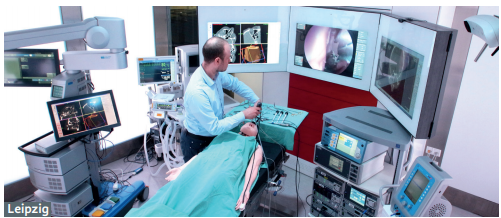
\includegraphics[scale = 0.8]{Content/Pictures/ornet.png}
	\caption{Operationssaal zur Demonstration von OR.NET in Leipzig, der für die Kopf- und Halschirurgie ausgelegt wurde \cite{ORnetWebsite}.}
	\label{fig:ornet}
\end{figure}

\subsection{Medizinische Standards}

Zur Kompatibilität medizinischer Geräte und Systeme unterschiedlicher Hersteller wurden Standards definiert, die erläutert werden sollen.

Einer der am Weitesten verbreiteten Standards ist DICOM (Digital Imaging and COmmunications in Medicine). DICOM ist ein schnittstellenkompatibles Datenformat für die digitale medizinische Bildgebung. Es fungiert dabei als Bildformat, wird aber auch zum senden, verteilen und speichern medizinischer Bilderdateien verwendet die von den bildgebenden Geräten (wie CT, MRT, US,..) erzeugt werden. Dabei ist das Dateiergebnis unabhängig von Aufnahmegerät und Hersteller. DICOM ist darüber hinaus für die Darstellung der Bilder verantwortlich und ermöglicht nachträgliche Bildverarbeitung. Zusätzlich bietet dieser Standard Vorteile für die Dokumentation und Anzeige von medizinischen Bilddateien. So werden bei DICOM Dateien bis zu 65.536 (16 Bit) unterschiedliche Grauschattierungen unterstützt, wobei im Gegensatz dazu bei JPG nur 256 (8 Bit) möglich sind \cite{DICOM}. Das verhilft Details im aufgenommenen Bild korrekt darzustellen und für den Chirurgen erkenntlich zu machen. Zu jeder aufgenommenen Bilddatei werden Daten, wie die Patienteninformationen oder Position des bildgebenden Geräts während der Aufnahme, gespeichert \cite{DICOM}.

Ein weiterer Standard ist HL7 (Health Level Seven). HL7 ist ein schnittstellenkompatibler Kommunikationsstandard wie DICOM \cite{DerDigitaleOperationssaal}. Dieser bietet Protokolle für den Austausch, die Integration, Abfrage und Organisation von digitalen Gesundheitsinformationen, die keine Bilddateien sind. Es wird festgelegt, mit welcher Sprache, Struktur und welchen Datentypen Informationen in Pakete verpackt und versendet werden \cite{HL7}.

PACS (Picture Archiving Communication System) ist zur Darstellung, Analyse, Manipulation und zur Langzeitarchivierung der Bild- und Patientendaten. Nachdem die Daten von einem Gerät erfasst werden, stehen sie im Netzwerk zur Verfügung und können von mehreren Zugriffspunkten eingesehen werden \cite{PACS}.
Die Bilder im DICOM Format werden über das DICOM Netzwerk übertragen und von PACS als DICOM Objekte komprimiert und archiviert \cite{DICOM}.

Die genannten Standards weisen im Zusammenspiel Limitierungen auf. Aus diesem Grund wurde IHE (Integrating the Healthcare Enterprise) entwickelt. IHE baut auf Standards wie DICOM und HL7 auf und soll das Zusammenwirken sowie die Kommunikation unterschiedlicher IT-Systeme im medizinischen Umfeld verbessern \cite{DICOMundIHE}. 
IHE ist eine Initiative von Gesundheitsexperten einen weiteren Kommunikationsstandard zu entwickeln, um die Art und Weise zu verbessern, wie Computersysteme miteinander interagieren und Informationen austauschen. Mit diesem Standard wird die Kommunikation zwischen unterschiedlichen Systemen verbessert, ist einfacher zu implementieren und ermöglicht Informationen effektiver zu nutzen \cite{IHE}.

Die Kombination der genannten Standards kann die Kompatibilität herstellerübergreifender Geräte und Systeme realisieren. 
Die Ausstattung eines OP-Saals kann somit flexibel ausgewählt werden \cite{DerDigitaleOperationssaal}.

\subsection{Sicherheitsprobleme und Datenschutz}

Mit der Digitalisierung und Vernetzung der Geräte und Systeme im Operationssaal, ist die Gewährleistung der Sicherheit und des Datenschutzes ein wichtiges Thema geworden.
Durch die Einbindung der medizinischen Geräte in das Netzwerk, sind diese neuen Gefahren ausgesetzt und es müssen Schutzmaßnahmen ergriffen werden. Wie bereits in der SOA erläutert, findet jegliche Kommunikation über den Operationssaal hinaus über ein Gateway statt. Eine Firewall wird eingesetzt, um den Datenverkehr zwischen dem OP- und Klinik-Netzwerk zu überwachen und gegebenenfalls Angriffe von außerhalb abzuwehren. Zur Gewährleistung von Sicherheit und Datenschutz muss auch sichergestellt werden, dass \glqq ein Medizingerät nur authentisierte, verifizierte und validierte Befehle entgegennimmt und ausführt\grqq{} \cite{DerDigitaleOperationssaal}. \\
Besonders im Bezug auf Datenschutz ist eine \glqq vertrauliche Übermittlung von sensiblen Daten wie Patientenidentität, Vitalparameter, Krankengeschichte und Medikation unerlässlich\grqq{} \cite{DerDigitaleOperationssaal}. Deshalb müssen die Geräte und Daten vor unerlaubten Lese- und Schreibzugriffen geschützt werden. \\
Die übermittelten Dateiformate bieten von sich aus keine Schutzmechanismen. Das wird deutlich, wenn eine DICOM Datei in einem Editor wie Wordpad betrachtet wird. Private und sensible Daten, wie den Patientennamen, behandelnden Arzt und das Krankenhaus, sind öffentlich lesbar und änderbar (Abb. \ref{fig:dicom}). Darüber hinaus kann das DICOM Bild mit passender Software betrachtet, bearbeitet oder ausgetauscht werden \cite{DICOM}.\\

Aus diesem Grund müssen das Netzwerk und die versendeten Daten vor unberechtigtem Zugriff und Manipulation geschützt und gegebenenfalls anonymisiert werden. Konkret findet jegliche Kommunikation über ein VPN (Virtual Private Network) statt und alle Computer im Netzwerk sind mit einer Firewall ausgestattet. Zur Sicherstellung von Integrität und Vertraulichkeit werden alle Nachrichten signiert und verschlüsselt \cite{DerDigitaleOperationssaal}. Darüber hinaus wir vor jeden Lese- und Schreibzugriff, das Zugriffsrecht validiert \cite{DICOM}.

Datenschutz muss in allen Bereichen der digitalen Medizintechnik gewährleistet und sichergestellt werden. Übergreifend ist damit nicht nur PACS und DICOM bzw. ersatzweise HL7 betroffen, sondern auch Radiologische Informationssysteme (RIS) und Krankenhaus Informationssysteme (HIS) \cite{DICOM}. 

\begin{figure} [t!]
	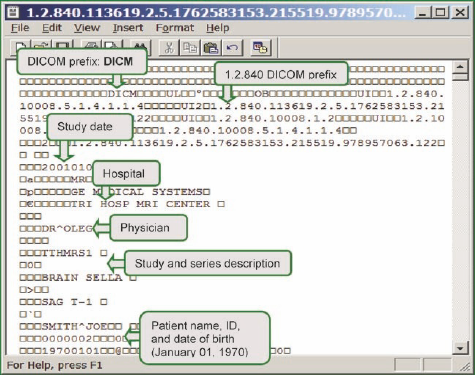
\includegraphics[scale = 0.7]{Content/Pictures/DICOMEditor.png}
	\caption{DICOM Datei in WordPad aus der Patienteninformationen, Krankenhaus und behandelnder Arzt direkt ausgelesen werden können \cite{DICOM}.}
	\label{fig:dicom}
\end{figure}

\chapter{\iflanguage{ngerman}{Herausforderungen}{Challenges}}
\label{sec:overview}

Der Hybride OP-Saal bringt Vorteile für die zukünftige Entwicklung des OP-Saals. Bei der Planung, Umsetzung und Vernetzung kommen Herausforderungen auf, die bewältigt werden müssen. Nicht alle Aspekte sind positiv und es soll validiert werden, ob sich ein Hybrider OP-Saal tatsächlich lohnt.

\subsection{Nachteile}

\begin{figure} [H]
	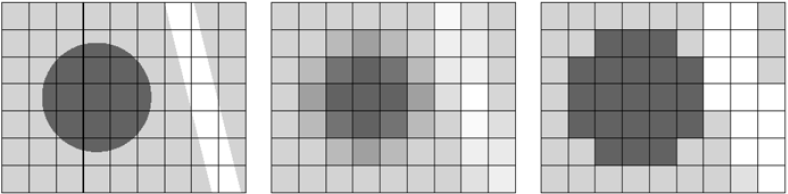
\includegraphics[scale = 0.7]{Content/Pictures/partial.png}
	\caption{Beispiel für Partialvolumenartefakte: (links) Abbild eines Tumors, (mitte) das finale Bild und (rechts) alle Voxel in denen Grauwerte des Tumors verzeichnet wurden \cite{DerDigitaleOperationssaal}.}
	\label{fig:partial}
\end{figure}

Der Hybride OP-Saal wird in erster Linie durch die bildgebenden Verfahren definiert. Wie aus der Radiologie bekannt müssen auch mögliche \glqq Mess-, Rekonstruktions- und Modellierungsfehler berücksichtigt werden\grqq{} \cite{DerDigitaleOperationssaal}. So können Partialvolumenartefakte (siehe Abb. \ref{fig:partial}) Grund dafür sein, dass Tumore in der falschen Größe dargestellt oder kleine Läsionen (< 1cm) nicht in den CT-Bildern abgebildet werden. Diese Fehler müssen in der komplexen und zeitaufwendigen Operationsplanung und späteren Durchführung berücksichtigt werden \cite{DerDigitaleOperationssaal}.

Hinzu kommt, dass Operationen im Hybriden OP-Saal teilweise unter laufender Röntgenkontrolle stattfinden. Diese Strahlenbelastung betrifft nicht nur den Patienten, sondern das gesamte behandelnde Team. Dieses wird der durch den Patienten verursachten Streustrahlung ausgesetzt. Je nach Abstand, Winkel und Höhe zum Patienten während der Bildkontrolle wird eine anwesende Person 9 bis 39\% der Strahlung ausgesetzt, die der Patient ausgesetzt wird \cite{RadiationExposure}. Abhängig von Größe und Gewicht des Patienten kann es aber auch zu einem höheren Streustrahlenanteil kommen und damit zu einer höheren Belastung für das behandelnde Team. Ist eine Person bei 100 Operationen mit je zwei 3D Scans pro Jahr anwesend, wird diese bereits 7\% der maximalen Jahresdosis ausgesetzt \cite{RadiationExposure}. Aus diesem Grund muss das Personal bei der Bildaufnahme hinter einer Strahlenschutzwand stehen oder wenn möglich den OP-Saal verlassen.

Ein anderes Problem entsteht bei der Tumorentfernung im Gehirn mit Hilfe von iMR. Um Veränderungen (wie Brain Shifts) frühzeitig erkennen und entsprechend reagieren zu können, sind regelmäßige Bildaufnahmen nötig. Für jede Bildaufnahme muss jedoch die Operation unterbrochen und ein Zeitaufwand für die Aufnahme aufgebracht werden \cite{BrainShiftInTumorResection}. Jede Aufnahme führt damit zu einer Verlängerung der Operationszeit und es muss ein Kompromiss zwischen Zeitaufwand und Bildhäufigkeit gefunden werden.\\
Alternativ kann stattdessen das US-Gerät verwendet werden. US ist aber im Gegensatz zu Magnetresonanztomografie nicht kontaktlos einsetzbar, was ein höheres Infektionsrisiko mit sich bringt \cite{BrainShiftInTumorResection}.

\subsection{Planung der Räumlichkeiten}

Die Raumplanung eines Hybriden OP-Saals ist ein komplexer Prozess (Abb. \ref{fig:roomplanning}), da er mehreren Fachbereichen gerecht werden muss. Die Bereiche haben unterschiedliche und teilweise sich gegenseitig ausschließende Ansprüche \cite{TechnicalConsiderations}. Aus diesem Grund müssen alle fachbereichsübergreifenden Chirurgen aber auch Anästhesisten, Arzthelfer und Techniker in den Planungsprozess miteinbezogen werden.
Durch die erhöhte Anzahl an Mitgliedern (8 bis 20 Personen) im Operationsteam ist eine Raumgröße von circa 70m² empfehlenswert. Mit Kontroll-, Technik- und Vorbereitungsraum müssen insgesamt mit circa 150m² gerechnet werden. Abhängig davon, ob die Geräte und Systeme wie der C-Bogen über eine Decken- oder Bodenbefestigung angebracht werden, müssen diese einem Gewicht von 650 bis 1800kg standhalten. Gleichzeitig dürfen die bildgebenden Systeme, Monitore, Beleuchtungsanlagen und das Personal nicht kollidieren. Durch die Raumgröße und Montage von Geräten an der Decke wird zusätzlich die Einhaltung der Hygienevorschriften erschwert \cite{TechnicalConsiderations}.\\ 
Aus den genannten Gründen muss normalerweise mit einer relativ langen Planungsphase für einen Hybriden OP-Saal gerechnet werden, um allen Ansprüchen einigermaßen gerecht zu werden und einen zukunftsfähigen OP-Saal zu errichten.

\begin{figure} [t!]
	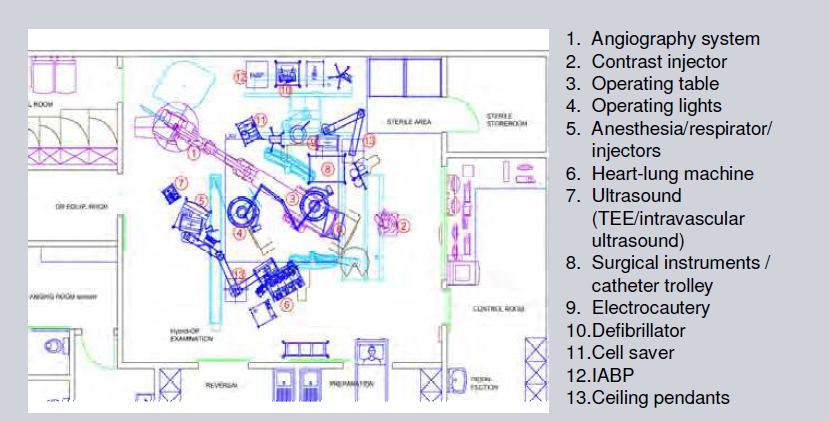
\includegraphics[scale = 0.7]{Content/Pictures/roomplanning.png}
	\caption{Beispielhaftes Layout für die Planung eines Hybriden OP-Saals \cite{HybridOR}.}
	\label{fig:roomplanning}
\end{figure}

\subsection{Kosten- Nutzen Verhältnis}

Eine der Fragen, die noch geklärt werden müssen, ist, ob ein Hybrider OP-Saal tatsächlich den Mehraufwand an Kosten und Umstrukturierung lohnt. Die benötigte Raumgröße und Ausrüstung führen dazu, dass ein Hybrider OP-Saal in der Anschaffung mehr als doppelt so teuer und in der Wartung fast doppelt so teuer wie ein Konventioneller OP-Saal ist \cite{HybridOR}. Gleichzeitig hat sich herausgestellt, dass neue medizinische Technologien positiv aufgenommen werden, obwohl ein Mehrwert dieser nicht bewiesen wurde. Dies und die Digitalisierung des Operationssaals haben in den letzten Jahren zu erheblichen Steigerungen der Gesundheitskosten beigetragen \cite{DerDigitaleOperationssaal}. \\
Welchen Mehrwert ein Hybrider OP-Saal tatsächlich bringt wird in Bezug auf Kosten und Operationszeit überprüft.

Im Anwendungsfall des Bauchaortenaneurysma konnte eine Operationszeiteinsparung von 23,5 Minuten (von 120 auf 96,5 Minuten) mit einem Hybriden OP-Saal gegenüber einem Konventionellen mit C-Bogen erreicht werden. Die Zeiteinsparung führt zu einer Einsparung der Prozesskosten um 276,17€ pro durchgeführter Operation. Bei dieser Studie wurde die Ergebnisse eines Hybriden OP-Saals von 2012 bis 2015 mit einem Konventionellen OP-Saal von 2007 bis 2012 verglichen. Im ersten Fall wurden Daten von 50 Patienten und im zweiten von 97 verwendet. Ein positiver Trend ist dennoch zu verzeichnen, da bei den Patienten und dem Operationsteam auf ähnliche Charakteristika geachtet wurde \cite{HybriderVsKonventioneller}.\\
Durch die Operationszeiteinsparung im Hybriden OP-Saal ist also tatsächlich eine Refinanzierung möglich \cite{HybriderVsKonventioneller}. Hinzu kommen positive Ergebnisse ohne direkten Vergleichswert, wie bei der Tumorentfernung. Bei 14 aus 16 Fällen konnten die Tumore komplett entfernt und auftretende Brain Shifts frühzeitig erkannt werden \cite{BrainShiftInTumorResection}.

Da Studien zum Vergleich von einem Hybriden und Konventionellen Operationssaal zum einen kaum vorliegen und zum anderen schwierig durchzuführen und zu validieren sind, lässt sich die Frage des tatsächlichen Nutzens sehr schwer beantworten. Auch der Vergleich von Todesraten ist kein aussagekräftiges Ergebnis, da Überleben auch mit Lebensqualität zusammenhängt\cite{HybriderVsKonventioneller}. \\
Weitere Faktoren, die einen Einfluss auf den Nutzen haben, sind die gefühlte und tatsächliche Sicherheit von Patienten und Chirurgen. Die psychologische Seite ist jedoch noch schwieriger zu bewerten als das tatsächliche objektive Ergebnis \cite{DerDigitaleOperationssaal}.

Trotzdem lässt sich festhalten, dass der Hybride OP-Saal seine Vorteile mit sich bringt. Nicht in allen medizinischen Bereichen wird er einen gleichgroßen Nutzen zur Geltung bringen, doch es eröffnen sich neue Möglichkeiten zur Operationsdurchführung \cite{ORofTheFuture}.





 






\chapter{\iflanguage{ngerman}{Zukünftige Entwicklung}{Development}}
\label{sec:overview}

In Science Fiction Filmen wie Transcendence wird die Zukunft des Operationssaals gerne mit vollautomatisierten Robotersystemen dargestellt, die innerhalb von Sekunden komplexe Eingriffe durchführen. 
Mit welchen Entwicklungen tatsächlich in naher Zukunft gerechnet werden kann und welche Sci Fi Ideen nicht so weit von der Wirklichkeit entfernt sind, soll in den folgenden Abschnitten erläutert werden.

\subsection{Neue Technologien}
Neue Technologien haben das Ziel, die Möglichkeiten im OP zu erweitern, mehr Sicherheit bzw. ein geringeres Risiko zu gewährleisten und das Team bei schwierigen Aufgaben zu unterstützen \cite{CurrentAndFuture}. 

Durch die Verbesserung der Bildqualität von Ultraschall (US) wird dieser in naher Zukunft vermehrt in OP-Sälen anzutreffen sein. Neue Möglichkeiten, wie der Aufnahme von dreidimensionalen Objekten (siehe Abb. \ref{fig:us}) in Echtzeit, eröffnen noch nicht dagewesene Anwendungsgebiete \cite{BrainShiftInTumorResection}. Hinzu kommen Möglichkeiten für die intravaskuläre Bildgebung, zur Aufnahme von Gefäßwänden mit an Kathetern befestigten US-Köpfen. Der Vorteil von US ist, dass gegenüber anderer Bildgebender Verfahren, weder der Patient noch das behandelnde Team radiologischer Strahlung ausgesetzt werden \cite{CurrentAndFuture}. Aus diesen Gründen und einer relativ guten Korrelation zwischen US- und MRT-Bildern, wird US auch in der Neuronavigation Anwendung finden \cite{BrainShiftInTumorResection}. \\
Bisher ist der Einsatz von Roboter- und Navigationssystemen im veränderlichen Körper begrenzt einsetzbar und noch in der klinischen Evaluation \cite{DerDigitaleOperationssaal}. Doch neue Funktionen wie Instrumentennavigation, Kollisionswarnungen und Neuromonitoring ermöglichen strahlenfreie Mikromanipulation, Navigation und Instrumentenführung. Besonders bei zeitaufwändigen komplexen Operationsvorgängen versprechen diese mehr Sicherheit und Kontrolle \cite{DerDigitaleOperationssaal,CurrentAndFuture}. \\
Bei derzeit in der Medizintechnik eingesetzten Robotersystemen handelt es sich meist um Master-Slave-Systeme. Also Systeme die vom Menschen gesteuert werden und mit denen bei komplexen Eingriffen über kleine Zugänge präzise gearbeitet werden kann. Aufgrund der vergleichsweise hohen Investitionskosten werden Robotersysteme in erster Linie für Eingriffe entwickelt, die der Chirurg ohne nicht ausführen könnte \cite{DerDigitaleOperationssaal}. Wie für das Operieren über natürliche Körperöffnungen. Erste Versuche wurden bereits mit dem Endosamurai (siehe Abb. \ref{fig:endosamurai}) der Olympus Deutschland GmbH durchgeführt. Gegenüber konventioneller Endoskope können mit dem Endosamurai über einen Zugang mit den Instrumentenarmen Zug- und Gegenkräfte aufgebracht werden \cite{Endosamurai,DerDigitaleOperationssaal}. 

Hinzu kommt eine standardisierten Vernetzung der Geräte und Systeme und herstellerübergreifende Kombinationslösungen. Ein übersichtliches Interface und zusätzliche Sprachsteuerung sollen zur Optimierung des chirurgischen Workflows beitragen. Die weitere Entwicklung in der computergestützten Optimierung der Visualisierung erlaubt zukünftig kontinuierliche Aufzeichnungen des Eingriffs \cite{DerDigitaleOperationssaal}. Daraus können Informationen zur automatisierten Operationsplanung für die individuelle Anatomie des Patienten gewonnen werden \cite{CurrentAndFuture}.

%\begin{figure} [H]
%	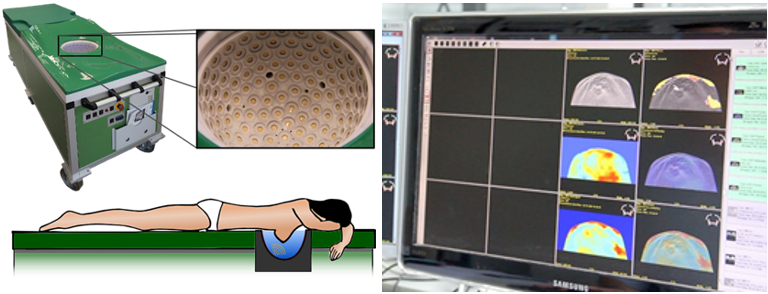
\includegraphics[scale = 0.5]{Content/Pictures/us.png}
%	\caption{(Links) Wassergefülltes Untersuchungsbecken für eine (rechts) %dreidimensionale Ultraschallaufnahme von der Brust zur Brustkrebsfrüherkennung %\cite{Ultraschall}.} 
%	\label{fig:us}
%\end{figure}

%\begin{figure} [H]
%	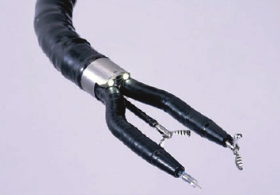
\includegraphics[scale = 0.7]{Content/Pictures/endo.png}
%	\caption{Endosamurai von der Olympus GmbH \cite{EndosamuraiBild}.} 
%	\label{fig:endosamurai}
%\end{figure}

\begin{figure}[!htb]
	\minipage{0.62\textwidth}
		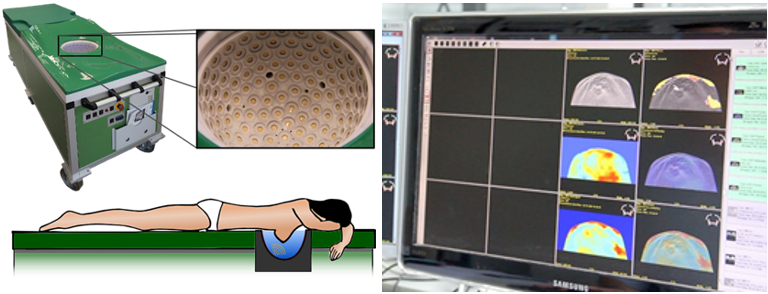
\includegraphics[width=\linewidth]{Content/Pictures/us.png}
		\caption{(Links) Wassergefülltes Untersuchungsbecken für eine (rechts) dreidimensionale Ultraschallaufnahme von der Brust zur Brustkrebsfrüherkennung \cite{Ultraschall}.} 
		\label{fig:us}
	\endminipage\hfill
	\minipage{0.35\textwidth}
		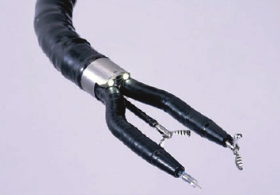
\includegraphics[width=\linewidth]{Content/Pictures/endo.png}
		\caption{Instrumentenarme des Endosamurai von der Olympus GmbH \cite{EndosamuraiBild}.} 
		\label{fig:endosamurai}
	\endminipage
\end{figure}

\subsection{Ausblick}
Wie sich der Operationssaal zukünftig entwickeln wird und welche Technologien von den theoretisch möglichen umgesetzt werden ist abhängig von den wirtschaftlichen Realitäten. Unabhängig davon, ist ein eindeutiger Trend in Richtung minimalinvasive Eingriffe zu verzeichnen. Dieser Trend wird durch die Entwicklungen in der Mikro- und Nanotechnik unterstützt und ermöglicht immer geringer belastendere Eingriffe \cite{DerDigitaleOperationssaal}. 

Monoport-Techniken und narbenlose Operationsverfahren über natürliche Körperöffnungen gewinnen zunehmend an Bedeutung. Zur Umsetzung dieser Entwicklung, müssen miniaturisierte Telemanipulationssysteme eingesetzt werden. Beispielsweise könnten autonome kabelgeführte Miniroboter über einen kleinen Zugang in den Körper eingeführt werden und sich selbständig zu einer bestimmten Position im Körper vorarbeiten. So könnte der Chirurg die Aufgabe der Navigation durch den Körper abgeben und mit am Katheter angebrachter miniaturisierte Visualisierungssysteme den Vorgang überwachen \cite{DerDigitaleOperationssaal}.\\
Eine andere vorstellbare Entwicklung könnte in Richtung eines minimierten Reinraums gehen. Dabei könnte in einer unsterilen Umgebung ein mit Vakuum fixierter Aufsatz über die Oberfläche des \glqq point of interest\grqq{} gestülpt und die Instrumente über einen Schleuse hindurchgeführt werden. Zur Umsetzung dieser Vision werden dann individualisierte \glqq single use\grqq{} Instrumente angefertigt und garantieren so eine optimale Abstimmung auf den Patienten und die Aufgabenstellung \cite{DerDigitaleOperationssaal}.

Die Mensch-Maschine-Interaktion spielt eine immer wichtigere Rolle und in der Zukunft wird das Zusammenspiel aus Bildgebenden Verfahren, Navigation, Robotik, IT und Benutzerinteraktion perfektioniert \cite{CurrentAndFuture}.
Auch heute schon ist der Hybride OP-Saal die Zukunft der Chirurgie \cite{Maquet}. Das wird sowohl den Patienten als auch den Chirurgen und dem Team zu Gute kommen.


	
	





\bibliography{Bibliography/thesis}


\end{document}
